
\documentclass[border=8pt, multi, tikz]{standalone} 
\usepackage{import}
\subimport{./layers/}{init}
\usetikzlibrary{positioning}
\usetikzlibrary{3d} %for including external image 

\def\ConvColor{rgb:yellow,5;red,2.5;white,5}
\def\ConvReluColor{rgb:yellow,5;red,5;white,5}
\def\PoolColor{rgb:red,1;black,0.3}
\def\BatchNormColor{rgb:blue,3; green, 1}
\def\DropoutColor{rgb:blue,1; green, 4; black, 0.1}
\def\UnpoolColor{rgb:blue,2;green,1;black,0.3}
\def\FcColor{rgb:blue,5;red,2.5;white,5}
\def\FcReluColor{rgb:blue,5;red,5;white,4}
\def\SoftmaxColor{rgb:magenta,5;black,7}   
\def\SumColor{rgb:blue,5;green,15}

\newcommand{\copymidarrow}{\tikz \draw[-Stealth,line width=0.8mm,draw={rgb:blue,4;red,1;green,1;black,3}] (-0.3,0) -- ++(0.3,0);}

\begin{document}
\begin{tikzpicture}
\tikzstyle{connection}=[ultra thick,every node/.style={sloped,allow upside down},draw=\edgecolor,opacity=0.7]
\tikzstyle{copyconnection}=[ultra thick,every node/.style={sloped,allow upside down},draw={rgb:blue,4;red,1;green,1;black,3},opacity=0.7]

\node[canvas is zy plane at x=0] (temp) at (-3,0,0) {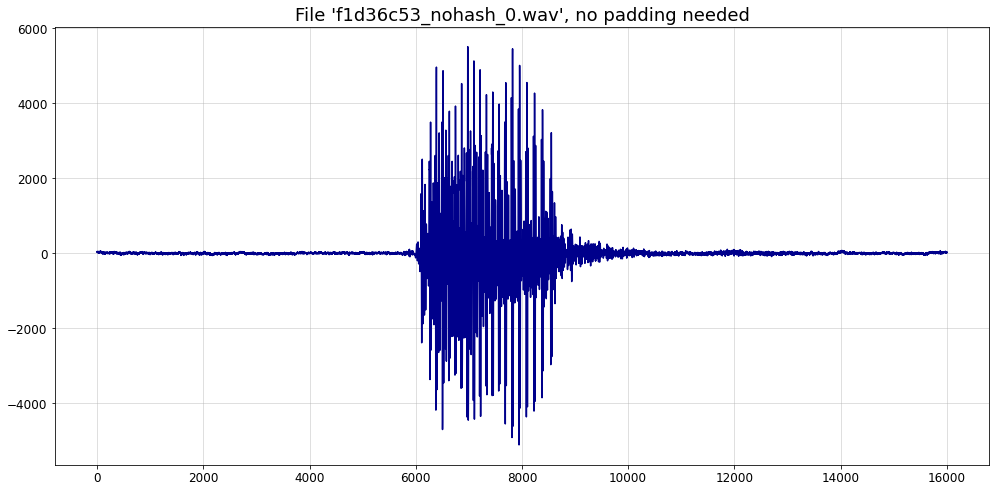
\includegraphics[width=21cm,height=8.4cm]{./examples/example1.png}};

\pic[shift={(0,0,0)}] at (0,0,0) 
    {RightBandedBox={
        name=convb1_1,
        caption= ,
        xlabel={{32, }},
        zlabel=,
        fill=\ConvColor,
        bandfill=\ConvReluColor,
        height=40,
        width=2,
        depth=100
        }
    };

\pic[shift={(0,0,0)}] at (convb1_1-east) 
    {RightBandedBox={
        name=convb1_2,
        caption= ,
        xlabel={{64, }},
        zlabel={(99, 39)},
        fill=\ConvColor,
        bandfill=\ConvReluColor,
        height=40,
        width=4,
        depth=100
        }
    };

\pic[shift={ (0,0,0) }] at (convb1_2-east) 
    {Box={
        name=poolb1,
        caption=,
        fill=\PoolColor,
        opacity=0.5,
        height=10,
        width=4,
        depth=100
        }
    };

\pic[shift={ (0,0,0) }] at (poolb1-east) 
    {Box={
        name=bnormb1,
        caption=,
        fill=\BatchNormColor,
        opacity=0.5,
        height=10,
        width=4,
        depth=100
        }
    };

\pic[shift={ (0,0,0) }] at (bnormb1-east) 
    {Box={
        name=dropoutb1,
        caption=,
        fill=\DropoutColor,
        opacity=0.5,
        height=10,
        width=4,
        depth=100
        }
    };

\pic[shift={(3,0,0)}] at (dropoutb1-east) 
    {RightBandedBox={
        name=convb2_1,
        caption= ,
        xlabel={{64, }},
        zlabel=,
        fill=\ConvColor,
        bandfill=\ConvReluColor,
        height=10,
        width=4,
        depth=100
        }
    };

\draw [connection]  (dropoutb1-east)    -- node {\midarrow} (convb2_1-west);

\pic[shift={(0,0,0)}] at (convb2_1-east) 
    {RightBandedBox={
        name=convb2_2,
        caption= ,
        xlabel={{128, }},
        zlabel={(99, 39)},
        fill=\ConvColor,
        bandfill=\ConvReluColor,
        height=10,
        width=8,
        depth=100
        }
    };

\pic[shift={ (0,0,0) }] at (convb2_2-east) 
    {Box={
        name=poolb2,
        caption=,
        fill=\PoolColor,
        opacity=0.5,
        height=3,
        width=8,
        depth=3
        }
    };

\pic[shift={ (0,0,0) }] at (poolb2-east) 
    {Box={
        name=bnormb2,
        caption=GlobalMaxPooling,
        fill=\BatchNormColor,
        opacity=0.5,
        height=3,
        width=8,
        depth=3
        }
    };

\pic[shift={ (0,0,0) }] at (bnormb2-east) 
    {Box={
        name=dropoutb2,
        caption=,
        fill=\DropoutColor,
        opacity=0.5,
        height=3,
        width=8,
        depth=3
        }
    };

\pic[shift={(1,0,0)}] at (dropoutb2-east) 
    {Box={
        name=convb3_1,
        caption= ,
        xlabel={{128, }},
        zlabel=,
        fill=\ConvColor,
        height=3,
        width=8,
        depth=3
        }
    };

\draw [connection]  (dropoutb2-east)    -- node {\midarrow} (convb3_1-west);

\pic[shift={(0,0,0)}] at (convb3_1-east) 
    {Box={
        name=convb3_2,
        caption= ,
        xlabel={{35, }},
        zlabel=,
        fill=\ConvColor,
        height=3,
        width=2,
        depth=3
        }
    };

\end{tikzpicture}
\end{document}
